\chapter{The domain matrices}
The domain matrices $\X{}$ and $\Y{}$ conjure considerable mystery. However under closer inspection we that they have elementary interpretations of unitary matrices. These domain matrices can be classified further as one of these types:
\begin{enumerate}
\item rotators
\item minimal spanning sets (bases)
\item reflections
\item permutations
\end{enumerate}

In the following sections we will discuss basic properties of unitary matrices then explore the different categories. 

The following chapters uses the Jordan normal form as a vehicle to probe these domain matrices.

Unitary matrices do not change the norm of a vector in $L_{2}$

Or course the product of unitary matrices are unitary.

\section{Unitary matrices}

Unitary matrices are easy to work with.
two views: a set of basis vectors, a process
unitary, orthogonal
\begin{equation}
  \U{}\U{*} = \I{}
\end{equation}
or
\begin{equation}
  \U{-1} = \U{*}
\end{equation}
Idempotent, index $k=2$.

Perhaps too much detail

spheres into spheres

%%
\subsection[Products of unitary matrices]{Products of unitary matrices are unitary}

An important realization is that the product of unitary matrices is also unitary. We will see that by looking at domain matrices as products of elementary unitary forms the \svdp \ looks much simpler.

Consider two conformable unitary matrices $\U{}\in\cmplx{m\times m}$ and $\V{}\in\cmplx{m\times m}$. Is there product unitary also?

Define
\begin{equation}
  \W{} = \U{}\V{*}.
\end{equation}
The question we are asking is this: Does the matrix product
\begin{equation}
  \W{}\W{}^{*} = \W{}^{*}\W{} = \I{m}?
  \label{eq:domains:unitarytest}
\end{equation}

To be explicit we show
\begin{equation}
  \W{}^{*}= \paren{\U{}\V{*}}^{*} = \paren{\V{*}}^{*}\U{*} = \V{}\U{*}.
\end{equation}
This implies the following:
\begin{equation}
  \begin{split}
    \W{}\W{}^{*} &= \paren{\U{}\V{*}}\paren{\V{}\U{*}}\\
      &=\U{} \paren{\V{*}\V{}} \U{*}\\
      &= \U{}\,\U{*}\\
      &= \I{m}.
  \end{split}
\end{equation}
A similar process shows that
\begin{equation}
  \W{}^{*}\W{} = \I{m}.
\end{equation}
Therefore the criteria of equation \eqref{eq:domains:unitarytest} are satisfied. Therefore the product of two unitary matrices is unitary. Therefore the product of three or more matrices are unitary.

This shows that a unitary matrix may be the composition of other unitary matrices. The implication is that we may examine the domain matrices and reveal a composition of elementary processes.

\endinput
\section{Planar coordinate systems}
Let's discuss orthogonal coordinate systems in the plane.

%%%
\subsection{Chirality in the plane}
\index{chirality!planar coordinate systems, of}
Recall the right-hand rule\index{right-hand rule} for an $x-y-z$ coordinate system. Start at the origin with your right hand and point your hand in the direction of increasing $x$. Curl your fingers in the direction of increasing $y$. Your thumb points in the direction of increasing $z$.

If your thumb points in the direction of decreasing $z$, then you have a left-handed coordinate system. What, you may ask, does this have to do with planar coordinate systems where $z=0$? We can use this concept to describe the \textit{orientation} of the coordinate system, as when we classify normal vectors\index{normal vectors} as inwards or outwards. If the planar coordinate system is right-handed, then we shade the object in green. For a left-handed system the shading is red. If we see a patch shaded green, the normal points towards us; red means the normal points away. ``Green is up'' and ``red is down.''

To illustrate these ideas we will start with the letter ``F'' in our reference coordinate system. When the letter is green it was plotted in a right-handed system. When the letter has other orientations in the plane, but is still green then we still have a right-handed coordinate system. When the forms of the letter are red, we are in a left handed coordinate system.


One way to approach this topic is to think of your computer screen as a blank slate for an orthogonal coordinate system. You may put the origin in any of the four corners. Once you have selected a corner anchor the coordinate system by serving as the origin, the next choice is pick the direction of increasing $x$. There are two choices for each corner. This is a total of eight different coordinate systems: four corner choices $\times$ two orientations per corner.

Let's pick one option as a reference and compare the others against it. Fix the origin in the lower left-hand corner and let the direction of increasing $x$ be along the horizontal to the right, much like when we draw a plot in the plane.

To facilitate the visualization, the $x-$axis is drawn in black, the $y-$axis in blue. Draw an angular arc from $x$ to $y$, from black to blue. If the angle is counterclockwise, the coordinate system is right-handed. Clockwise angles signal a left-handed coordinate system. This scheme is used in table \eqref{tab:chiral:rotations}.

\begin{table}[htdp]
\begin{center}
\begin{tabular}{cc}
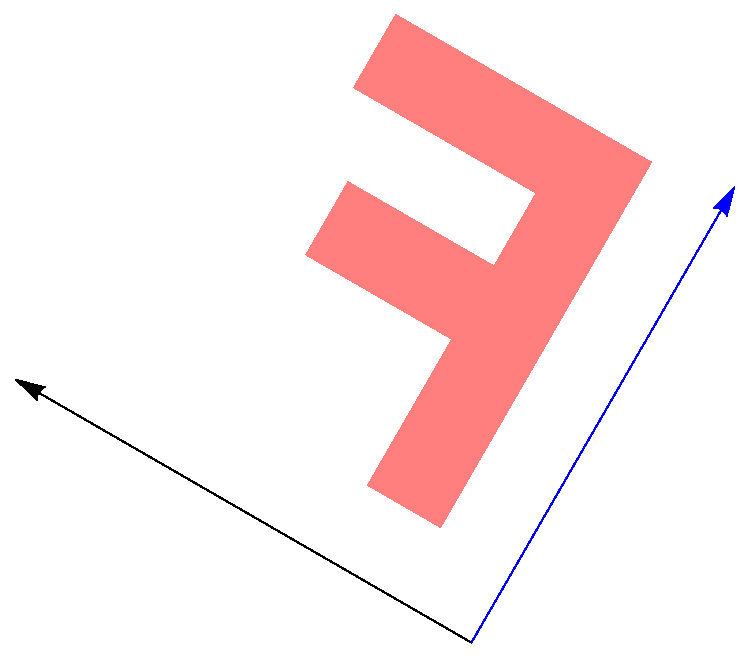
\includegraphics[ width = 2.25in ]{pdf/coordinate_systems/ref} &
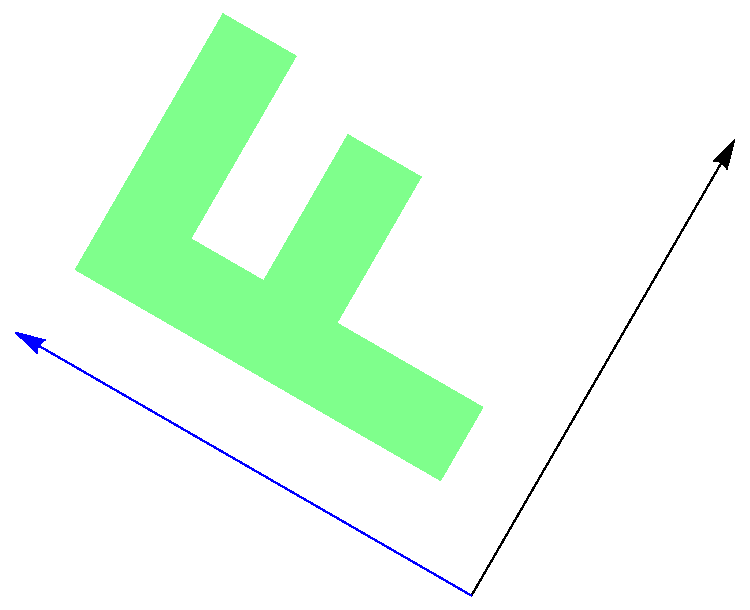
\includegraphics[ width = 2.25in ]{pdf/coordinate_systems/rot} \\[10pt]
left-handed system & right-handed system\\[5pt]
 $\ktwo\mat{rr}{\cos \theta & -\sin \theta \\ \sin \theta & \cos \theta}\xtwo$ & 
 $\mat{rr}{\cos \theta & -\sin \theta \\ \sin \theta & \cos \theta}\xtwo$ \\[20pt]
\end{tabular}
\end{center}
\caption{Sample rotations in the plane. The $x-$axis is shown in black, the $y-$axis in blue. To jump between these images think of reflection through the line $y=x$. As you can imagine, such a reflection would require that the figure be turned over, revealing the other size.}
\label{tab:chiral:rotations}
\end{table}%

\begin{table}[htdp]
\begin{center}
\begin{tabular}{l|ll}
 & right-handed & left-handed   \\\hline
 patch color    & green   & red \\\hline
 patch surface  & top & bottom  \\\hline
 surface normal & outward & inward \\\hline
 angle: $x$ to $y$ & counterclockwise & clockwise \\\hline
\end{tabular}
\end{center}
\label{tab:chiral:youarerighthandedif}
\caption{Different ways to express the same concept.}
\end{table}%

\begin{table}[htdp]
\begin{center}
\begin{tabular}{m{1.75in}ll}
  \qquad image & \quad transformation & operation\\\hline
  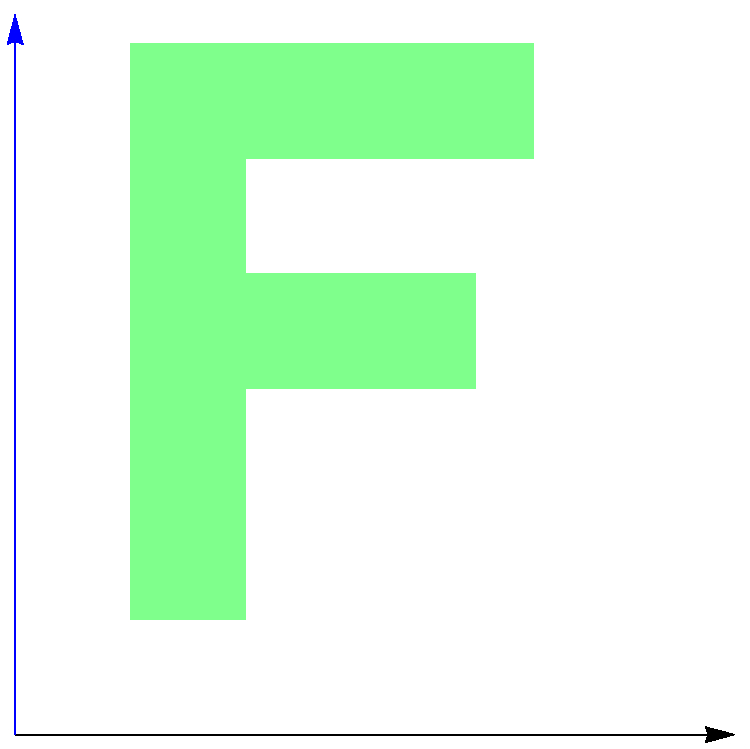
\includegraphics[ width = 1.5in ]{pdf/coordinate_systems/Ia}   & $\itwo\xtwo=\mat{r}{x\\y}$ & identity\\\hline
  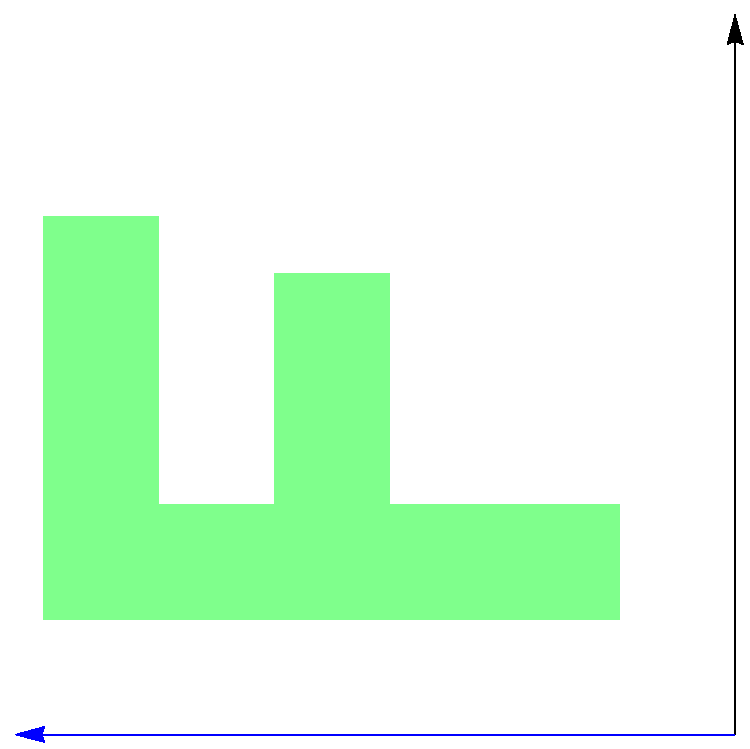
\includegraphics[ width = 1.5in ]{pdf/coordinate_systems/IIa}  & $\mat{rr}{0&1\\-1&0}\xtwo=\mat{r}{y\\-x}$ \qquad & rotation by $\pi/4$ \\\hline
  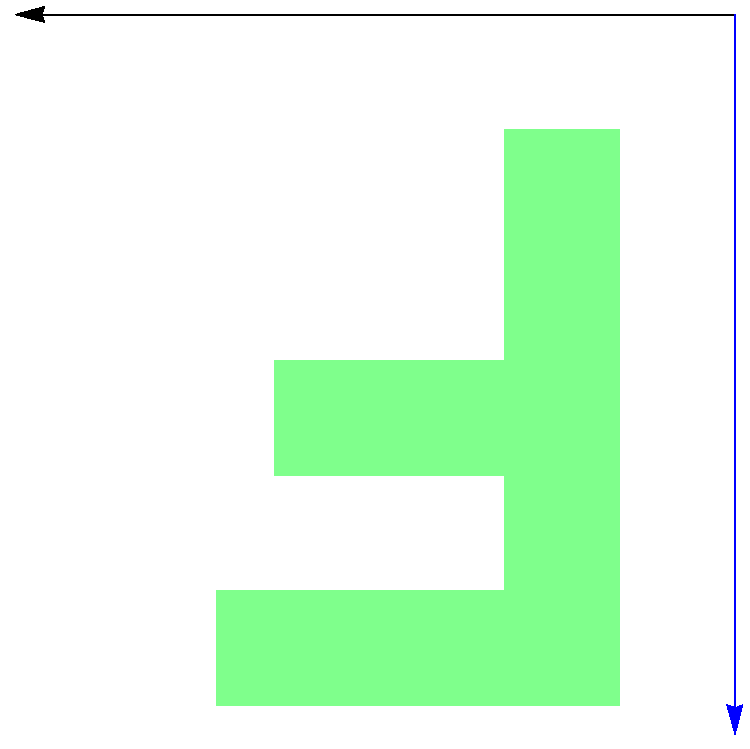
\includegraphics[ width = 1.5in ]{pdf/coordinate_systems/IIIa} & $\mat{rr}{-1&0\\0&-1}\xtwo=\mat{r}{-x\\-y}\qquad$ \qquad & rotation by $\pi/2$ \\\hline
  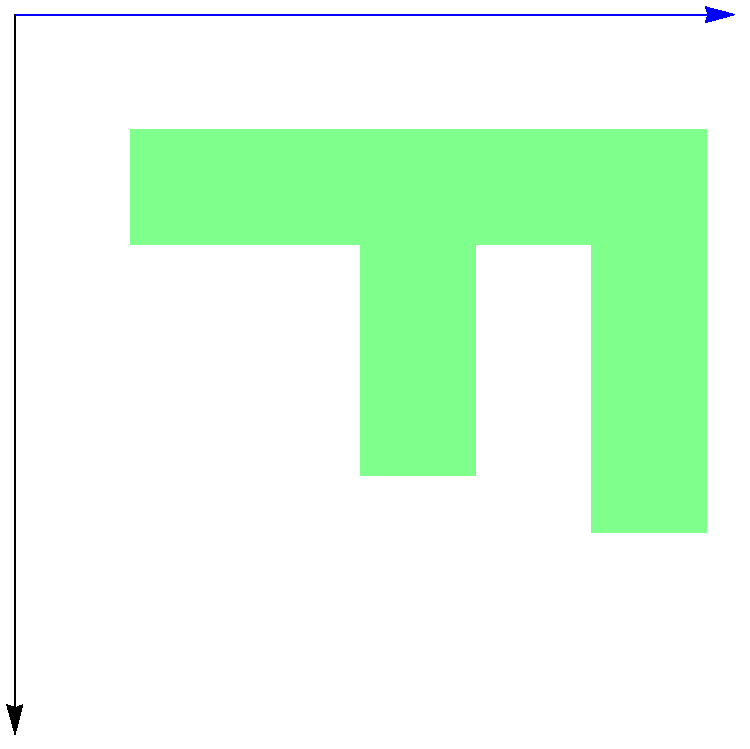
\includegraphics[ width = 1.5in ]{pdf/coordinate_systems/IVa}  & $\mat{rr}{0&-1\\1&0}\xtwo=\mat{r}{-y\\x}$ \qquad & rotation by $3\pi/4$ \\\hline
\end{tabular}
\end{center}
\label{tab:chiral:right}
\caption{Right-handed coordinate transformations. Think of the letter ``F'' as being composed of discrete points. The matrix operations show how each point is transformed in each of the images. Notice that in all cases the angular arc connecting the $x-$axis to the $y-$axis is $\pi/4$ counterclockwise.}
\end{table}%

\begin{table}[htdp]
\begin{center}
\begin{tabular}{m{1.75in}ll}
  \qquad image & \quad transformation & operation\\\hline
  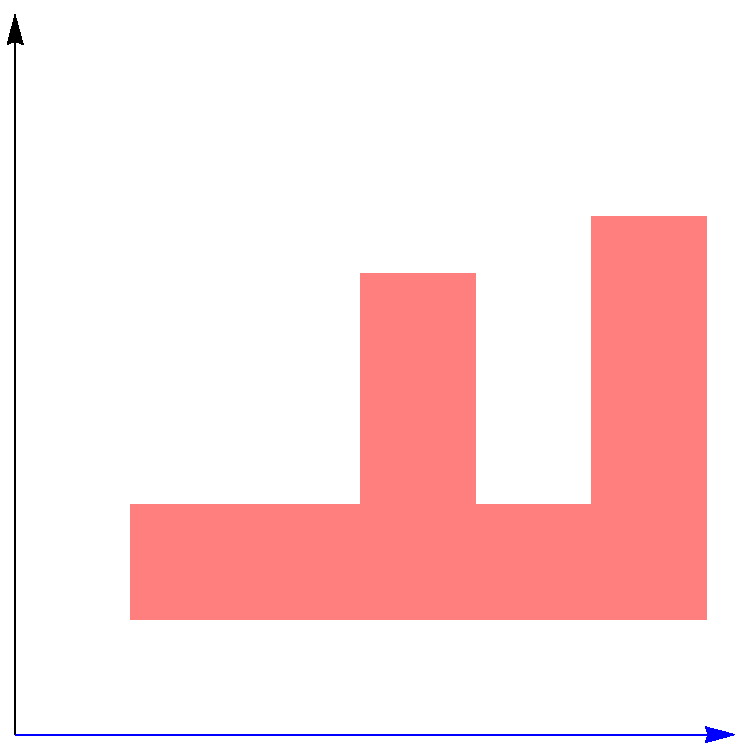
\includegraphics[ width = 1.5in ]{pdf/coordinate_systems/Ib}   & $\mat{rr}{0&1\\1&0}\xtwo=\mat{r}{y\\x}$ & reflect through $y=x$\\\hline
  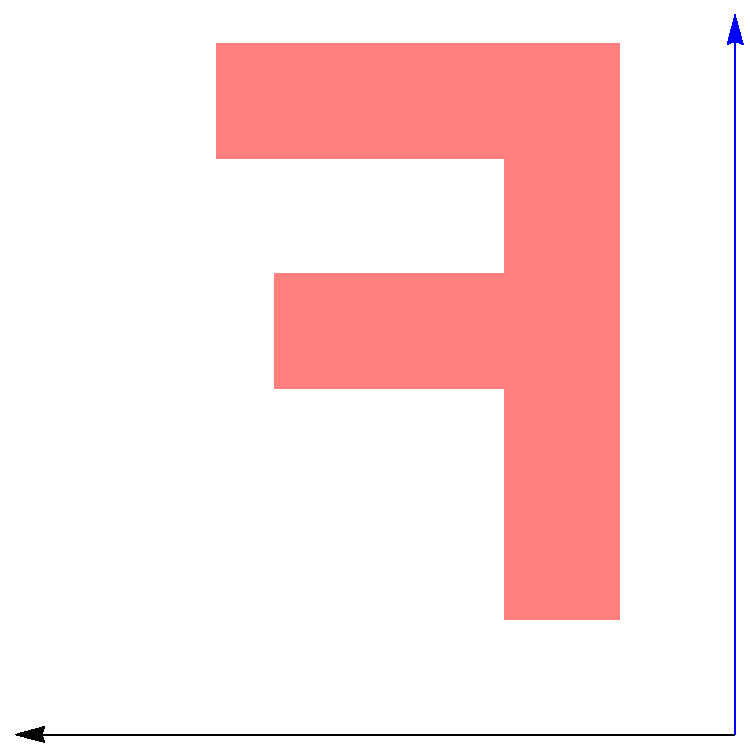
\includegraphics[ width = 1.5in ]{pdf/coordinate_systems/IIb}  & $\mat{rr}{0&1\\-1&0}\xtwo=\mat{r}{y\\-x}$ \qquad & rotation by $\pi/4$ \\\hline
  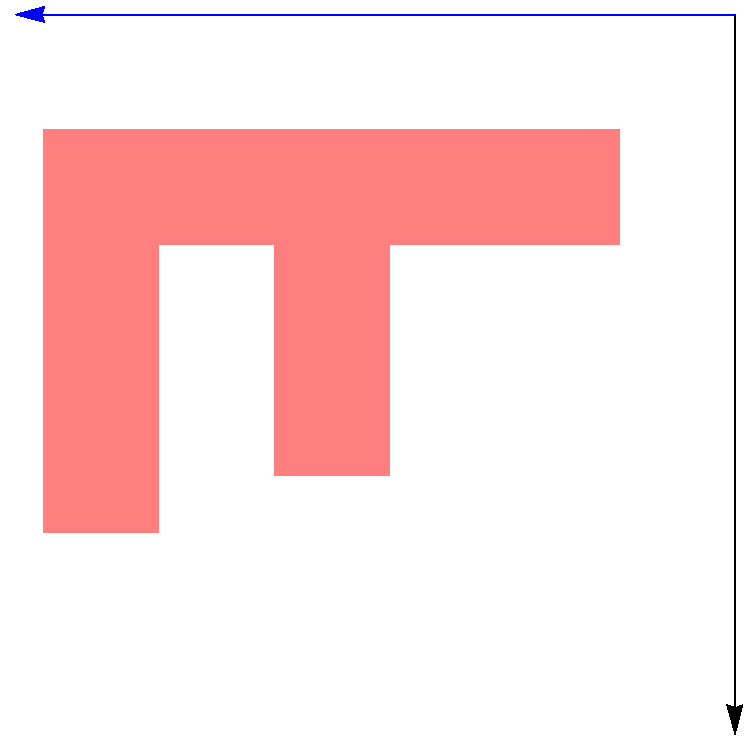
\includegraphics[ width = 1.5in ]{pdf/coordinate_systems/IIIb} & $\mat{rr}{-1&0\\0&-1}\xtwo=\mat{r}{-x\\-y}\qquad$ \qquad & rotation by $\pi/2$ \\\hline
  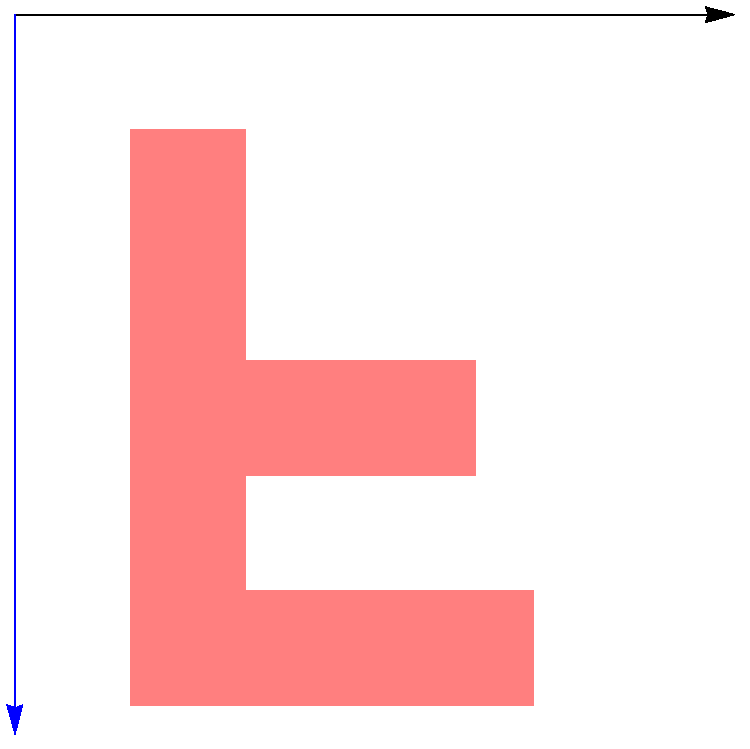
\includegraphics[ width = 1.5in ]{pdf/coordinate_systems/IVb}  & $\mat{rr}{0&-1\\1&0}\xtwo=\mat{r}{-y\\x}$ \qquad & rotation by $3\pi/4$ \\\hline
\end{tabular}
\end{center}
\label{tab:chiral:left}
\caption{Left-handed coordinate transformations.}
\end{table}%

\endinput
%\input{chapters/bases/rotators}
%\input{chapters/bases/reflectors}
%% fundamental projectors
\def\projra {\mathbf{P}_{\rng{\A{}}}}
\def\projrap{\mathbf{P}_{\rng{\A{}}^{\perp}}}
\def\projna {\mathbf{P}_{\nll{\A{}}}}
\def\projnap{\mathbf{P}_{\nll{\A{}}^{\perp}}}

\def\projrat {\mathbf{P}_{\rng{\A{T}}}}
\def\projratp{\mathbf{P}_{\rng{\A{T}}^{\perp}}}
\def\projnat {\mathbf{P}_{\nll{\A{T}}}}
\def\projnatp{\mathbf{P}_{\nll{\A{T}}^{\perp}}}

\providecommand{\aap}[1]   {\Y{}\,\sig{}\,\sig{(+)}\,\Y{#1}}
\providecommand{\apa}[1]   {\X{}\,\sig{(+)}\,\sig{}\,\X{#1}}

%\providecommand{\pra}[1]   {\Y{}\,\J{m}{\rho}\Y{#1}}
%\providecommand{\pnap}[1]  {\X{}\,\J{n}{\rho}\,\X{#1}}

\providecommand{\pra}[1]   {\yrng{}\yrng{#1}}
\providecommand{\pnap}[1]  {\xrng{}\xrng{#1}}

\endinput
%\input{chapters/bases/bases}
%\input{chapters/bases/GroupTheory}


\endinput